\section{Introduction}

Ceci est le corps de mon document.
Je peux écrire du texte ici, et il sera affiché dans le document final.

\blindtext[1]


%\pagebreak

\section{Maths}

\subsection{Les maths de base}

On peut écrire des équations:
\blindtext

$$
    a x + b = 5
$$

\noindent On peut utiliser les symboles mathématiques:

\begin{equation}
    u_n = \int_{x=0}^\infty v^2(x) dx
    \label{eq:nice_one}
\end{equation}

On voit dans l'équation Eq. \ref{eq:nice_one} \footnote{voir page \pageref{eq:nice_one}} que la théorie est fausse.

\subsection{Les maths en ligne}

On peut intégrer des maths dans le texte, par exemple $\alpha = 5$ et $x = \frac{3}{4}$.
On remarque que ces résultats sont très importants.
On remarque que ces résultats sont très importants.

\subsection{Des maths un peu plus avancées}

On veut montrer des choses:

\begin{align}
    A & = \left( a + b\right)^2 \nonumber \\
      & = a^2 + 2 ab + b^2
\end{align}

On vous donne les valeurs suivantes:
\begin{itemize}
    \item La masse $m = \qty{5.01d23}{\kilo\gram}$.
    \item La vitesse
          $$
              v = \qty[per-mode=fraction]{5}{\meter\per\second}$$
    \item La pression:
          $$
              P = \qty{5}{\newton\per\meter\squared}
          $$
\end{itemize}

\section{Enumerations}

On peut énumérer:

\begin{enumerate}
    \item Point 1
    \item Point 2
\end{enumerate}

\section{Mise en page}

On peut utiliser FancyHDR pour modifier la mise en page du documen.
Pour aller plus loin, voir \href{https://fr.overleaf.com/learn/latex/Headers_and_footers#Using_the_fancyhdr_package}{lien}.
On peut aussi utiliser le package parindent pour modifier la forme des paragraphes \href{https://www.overleaf.com/learn/latex/Articles/How_to_change_paragraph_spacing_in_LaTeX#The_parskip_package}{(lien)}.
%paragraphes \href{https://www.overleaf.com/learn/latex/Articles/How_to_change_paragraph_spacing_in_LaTeX#The_parskip_package}{Overleaf}.

\section{Figures en \LaTeX}

On peut intégrer des images facilement avec 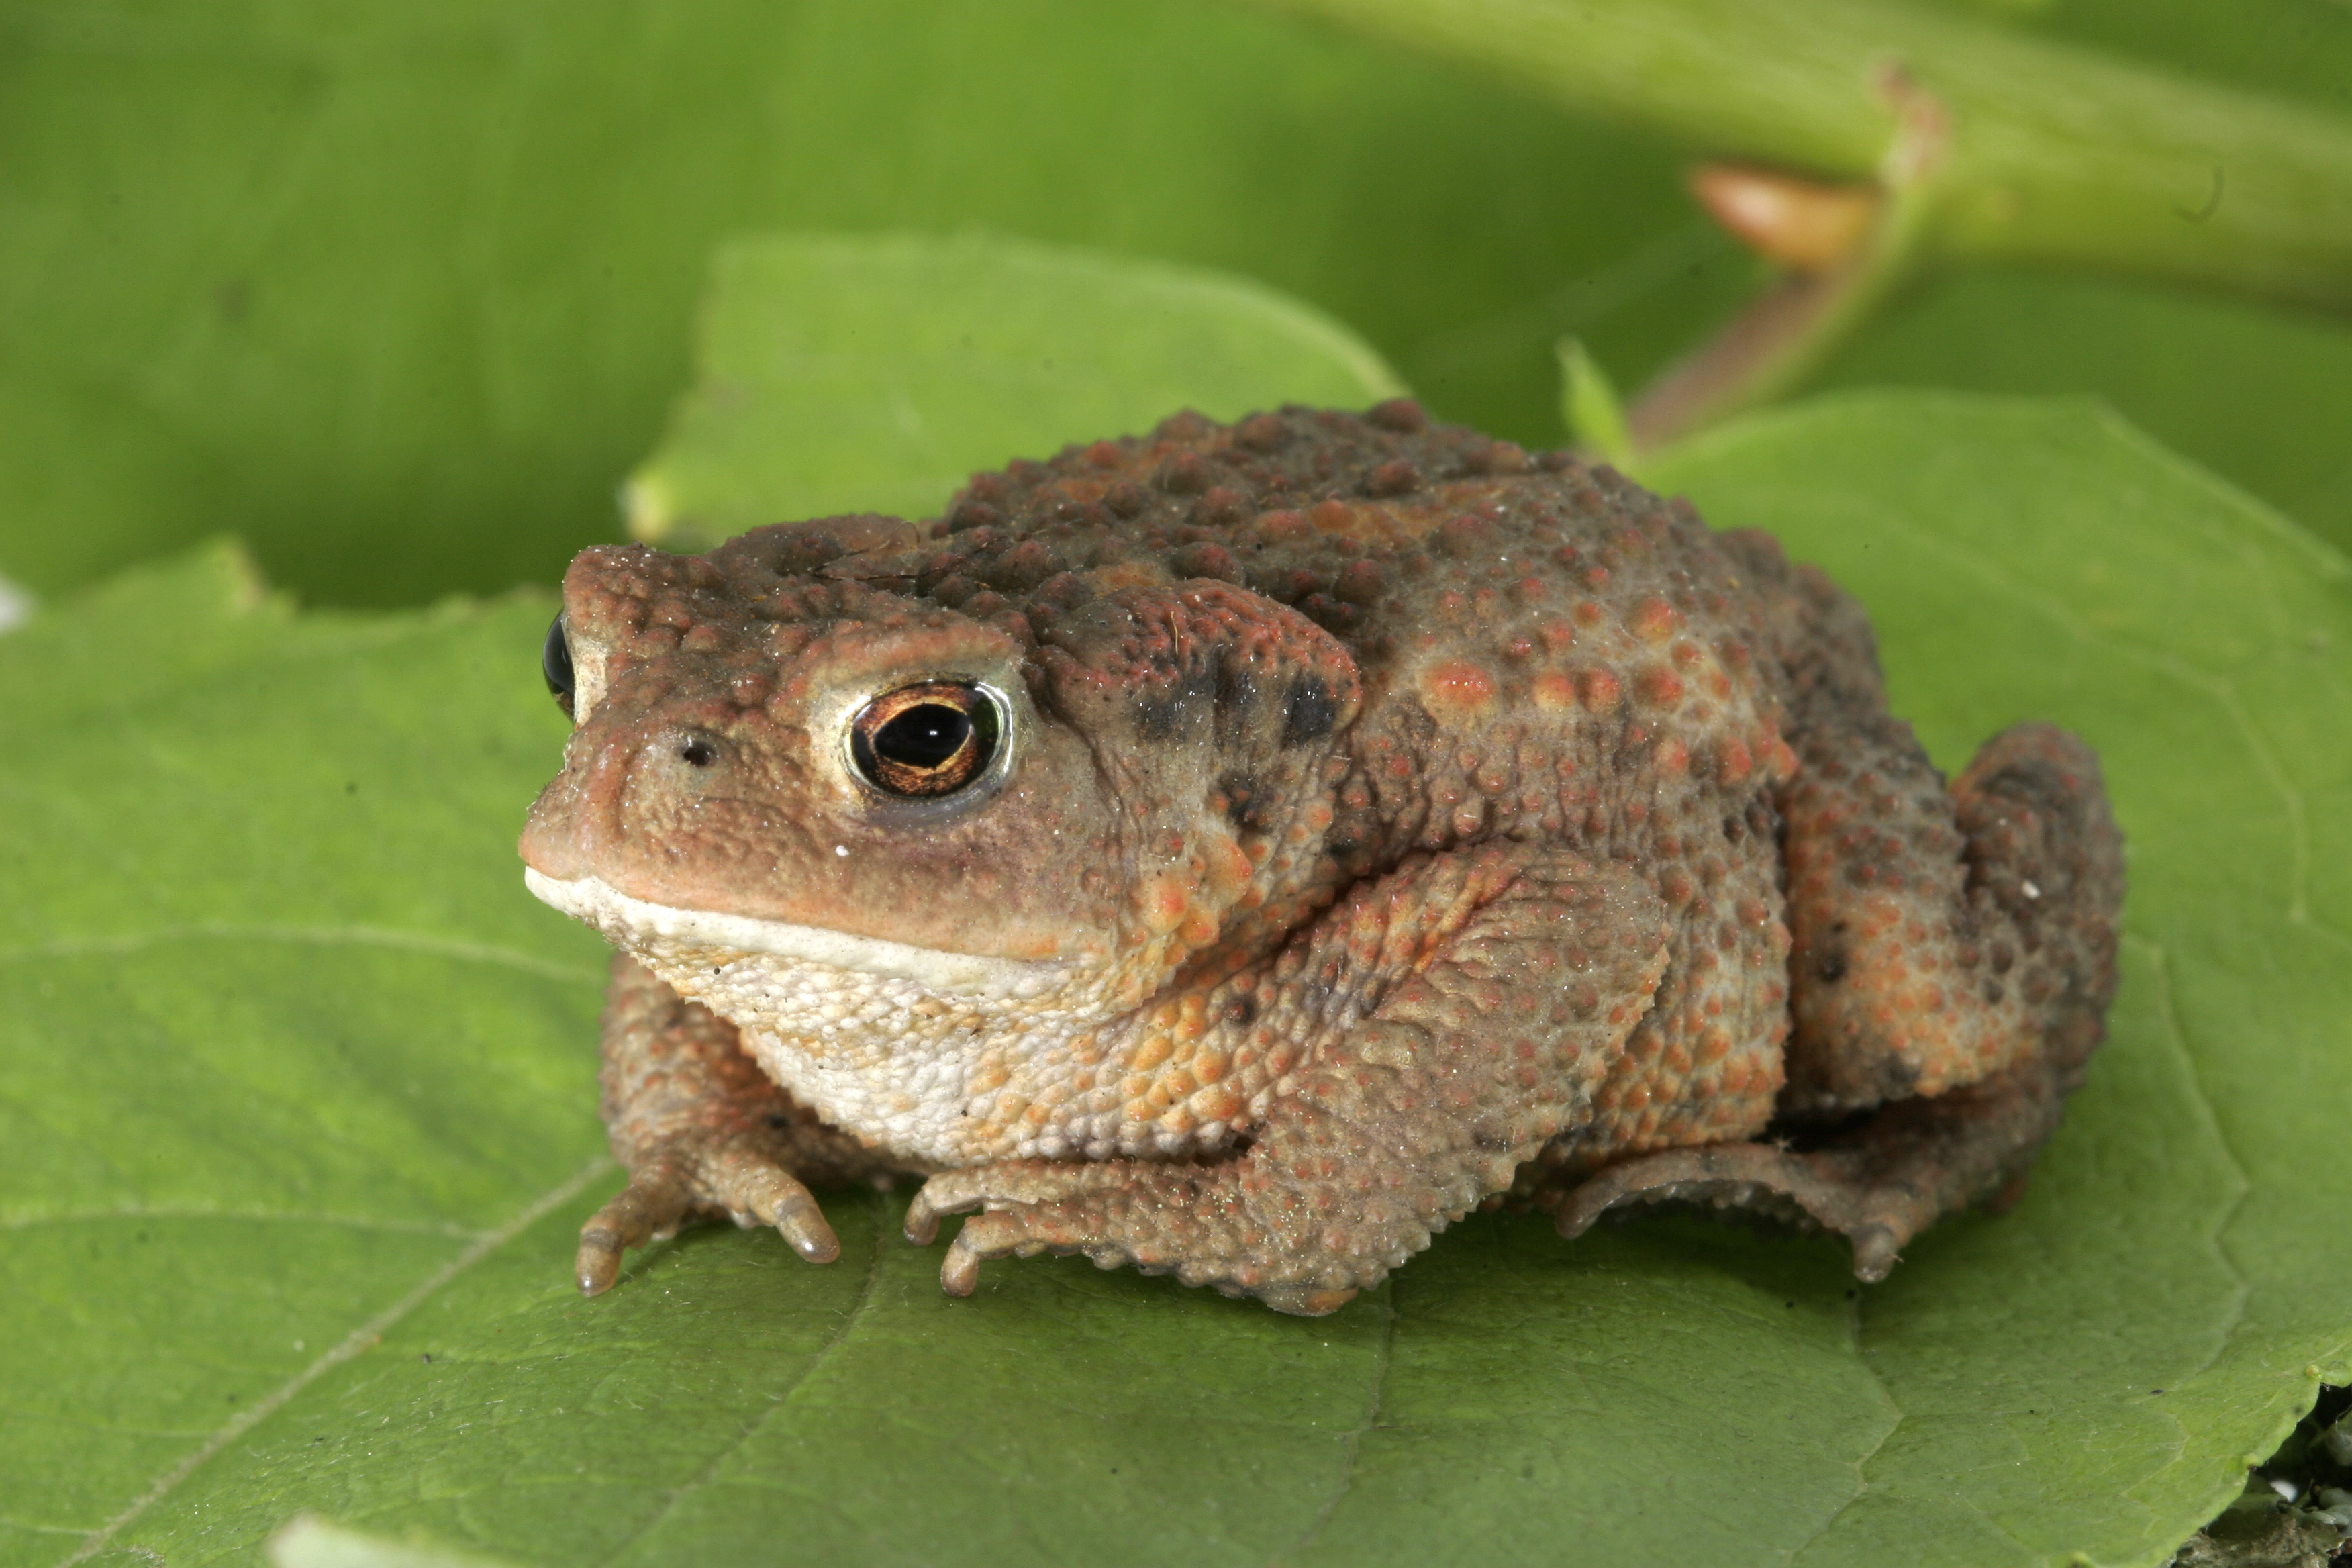
\includegraphics[width=12mm]{figures/toad.jpg}.

% EXEMPLE DE FIGURE
\blindtext[2]

\begin{figure}[htbp]
    \begin{center}
        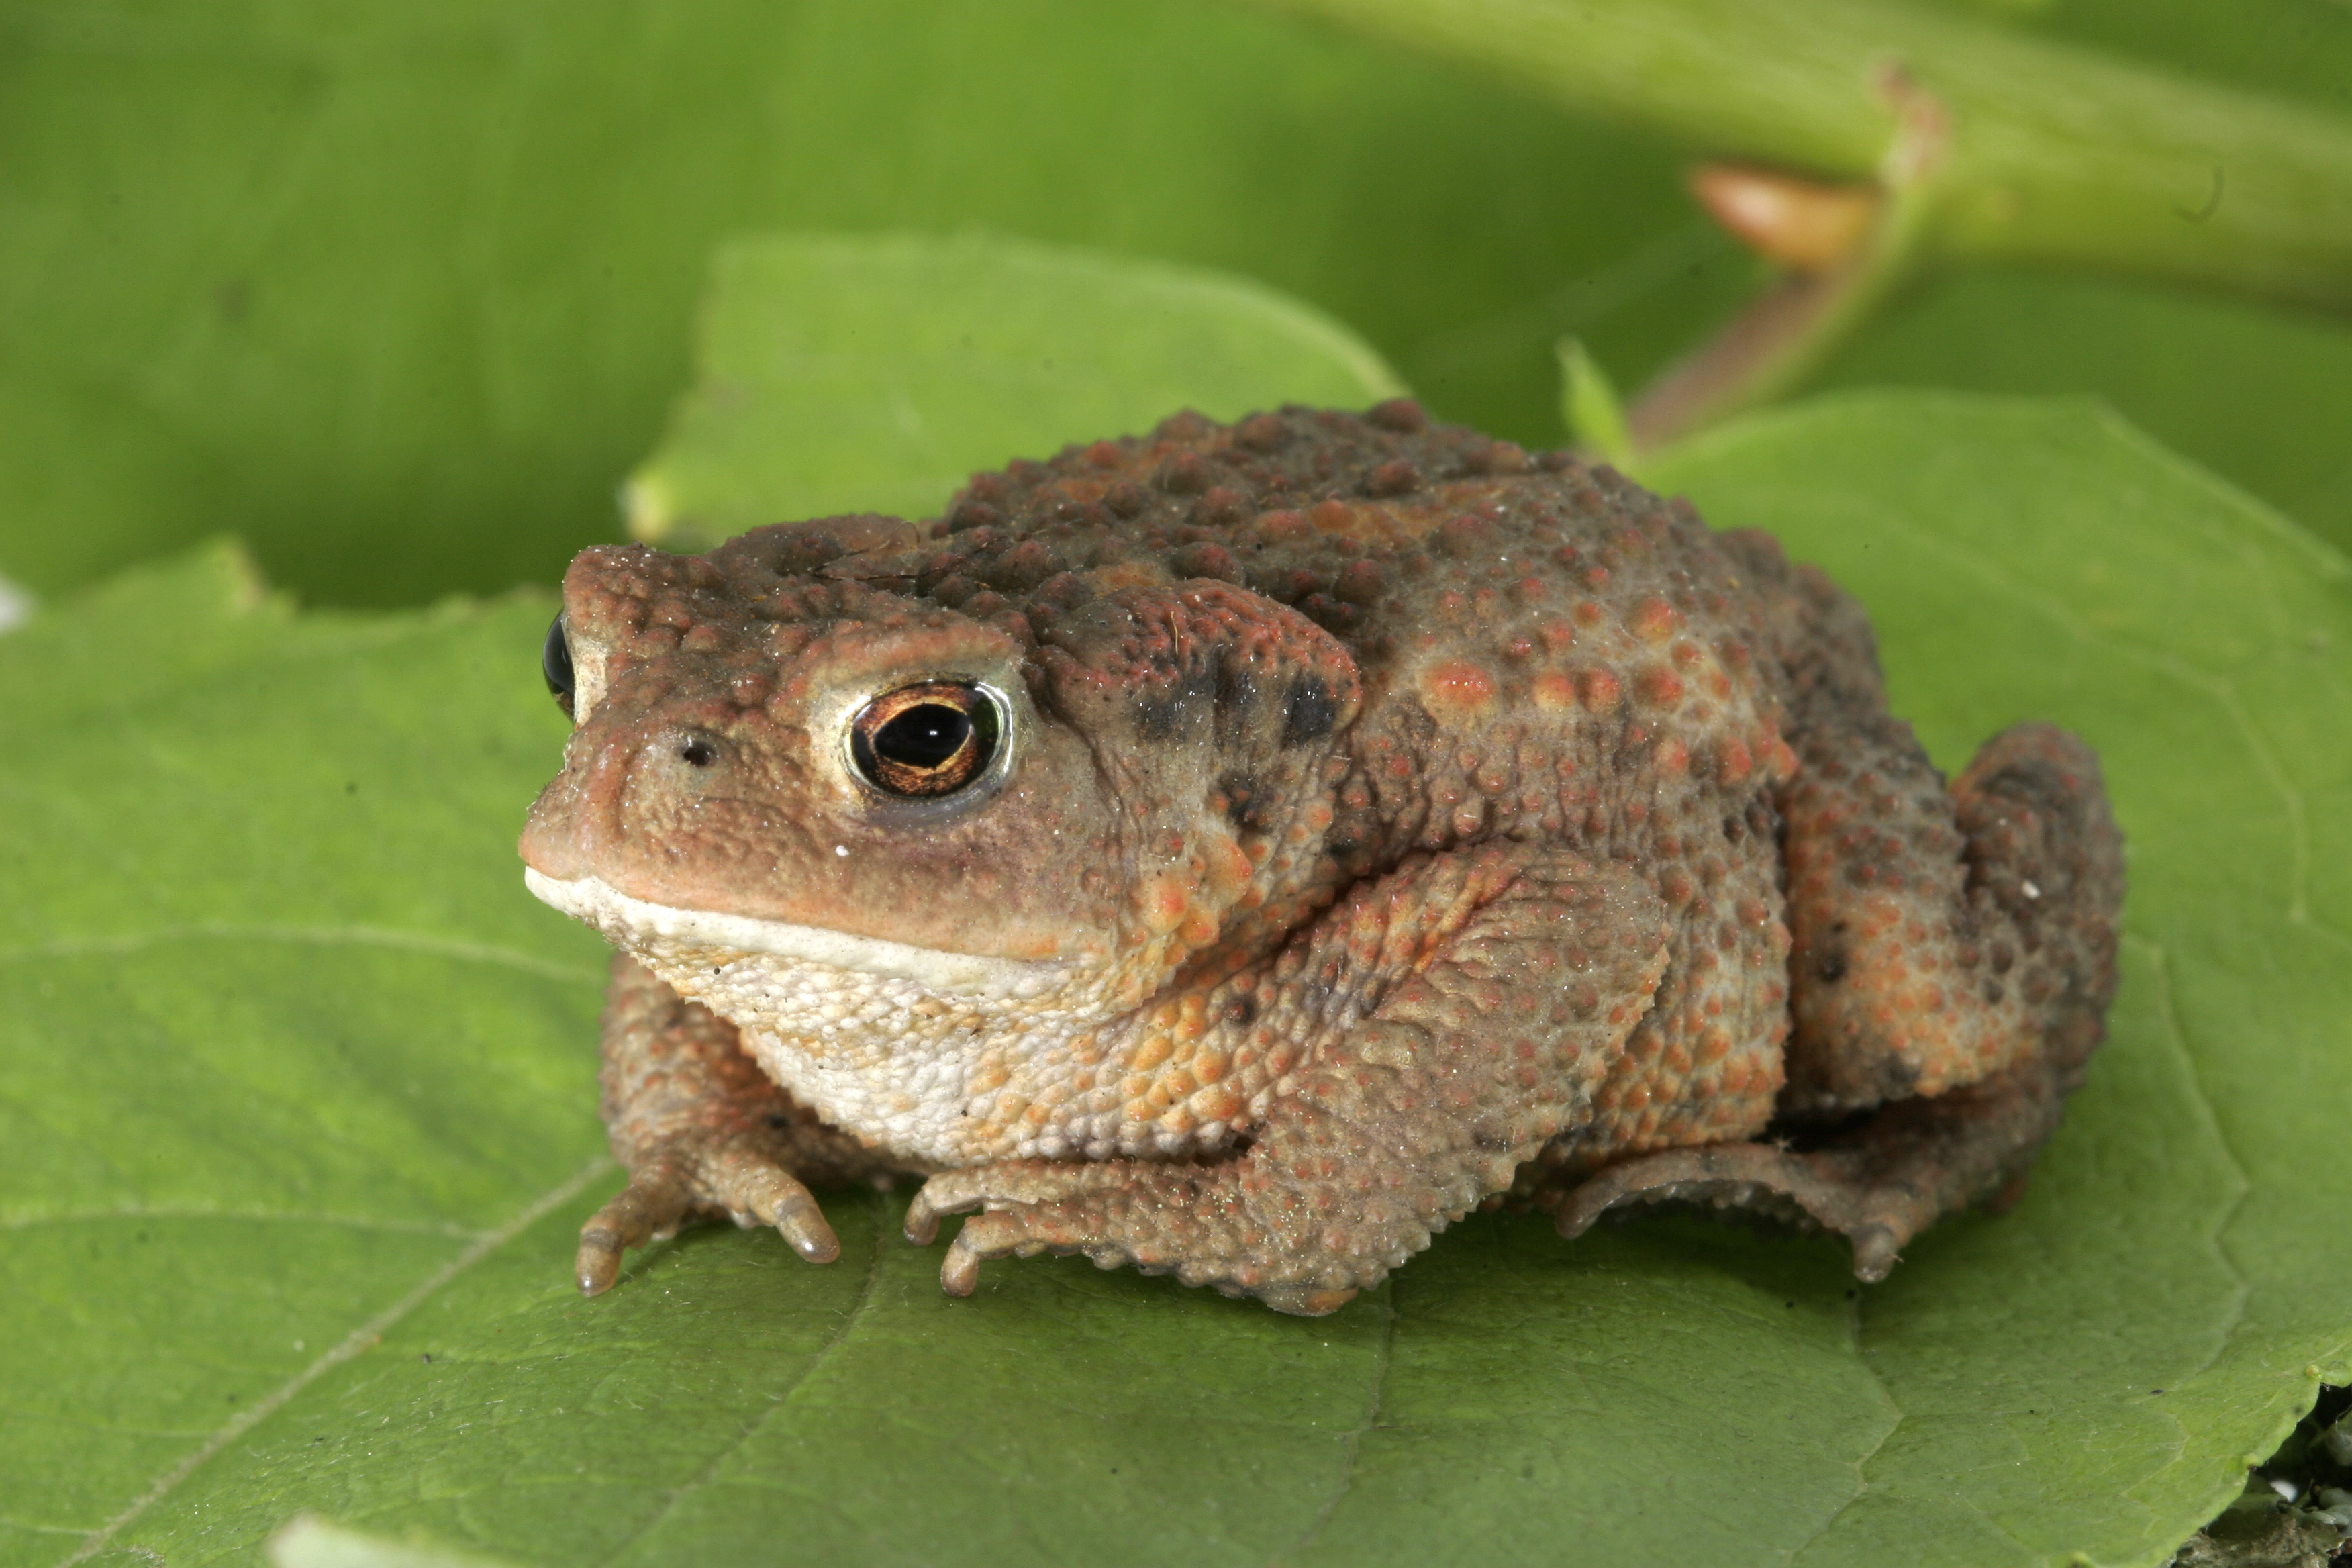
\includegraphics[width=1.\textwidth]{figures/toad.jpg}
    \end{center}
    \caption{Un superbe crapaud.}
    \label{fig:toad}
\end{figure}

On aurait pu penser que la figure serait là.
\blindtext[2]

\section{Tables et tableaux}

\begin{tabular}{ccc}
    a & b & c \\
    e & e & f
\end{tabular}

\begin{table}[]
    \caption{A nice table.}
    \label{tab:nice_table}
    \begin{center}
        \begin{tabular}{@{}lcr@{}}
            \toprule
            Name & Age & Address \\
            \midrule
            Bob & Bill  & 1 first street \\
            \bottomrule
        \end{tabular}
    \end{center}
    
\end{table}


\section{Citations de refs biblio}

On peut citer des reférences une par une \citep{hawking1974black}. 
On peut citer plusieurs articles à la fois \citep{belczynski2012missing,hawking1974black}.
Comme le dit très bien \citeauthor{belczynski2012missing}, on peut y arriver.